\chapter{精确解}
从问题中得出抽象的数学表达,得到方程~\eqref{equ:choux}:
\begin{equation}\label{equ:choux}
	\dfrac{\partial C}{\partial t}= \alpha\dfrac{\partial^2 C}{\partial x^2}-\beta\dfrac{\partial C}{\partial x}-\gamma C + \delta
\end{equation}
这是一个对流扩散反应方程。\par
参考表~\ref{tab:ne}~可以看到$\beta\gg\alpha$,故此方程为一个对流占优的对流扩散反应方程。\par
解这样的一个方程是困难的,我们首先解扩散方程,然后解对流方程,再尝试解对流——扩散——反应方程。
% \section{扩散方程}
% 考虑这样的一个方程,即方程~\eqref{equ:kuosan1}
% \begin{equation}\label{equ:kuosan1}
% 	\dfrac{\partial C}{\partial t}-a^2\dfrac{\partial^2 C}{\partial x^2}=0
% \end{equation}
% 它的定解条件为
% \begin{equation}
% \begin{aligned}\label{equ:kuosan_bianjie}
% C(x=0,t)&=0\\
% \left.\dfrac{\partial C}{\partial x}\right|_{x=L}&=0
% \end{aligned}
% \end{equation}
% \begin{equation}\label{equ:kuosan_chushi}
% \left.C(x,t)\right|_{t=0}=\psi(x)
% \end{equation}\par
% 泛定方程和边界条件都是齐次的,应用分离变数法,其试探解
% \begin{equation}
% 	C(x,t)=X(x)T(t)
% \end{equation}
% 代入方程~\eqref{equ:kuosan1}、~\eqref{equ:kuosan_bianjie},得
% \begin{equation}\label{equ:changX}
% 	\dfrac{\partial^2 X}{\partial x}+\lambda X=0
% \end{equation}
% \begin{equation}
% 	X(0)=0,X'(l)=0
% \end{equation}
% \begin{equation}
% 	\dfrac{\partial T}{\partial t}+\lambda a^2 T=0
% \end{equation}
% 考虑$\lambda$为实数的情况,当$\lambda$<0时,方程~\eqref{equ:changX}~的解为
% \begin{equation}
% 	X(x)=C_1e^{\sqrt{-\lambda}x}+C_2e^{-\sqrt{-\lambda}x}
% \end{equation}
% 积分常数$C_1$和$C_2$由条件~\eqref{equ:kuosan_bianjie}~确定,解得$X(x)=0$,这是没有意义的。\par
% 同样,当$\lambda$=0时$X(x)=0$,没有意义,我们来看$\lambda$>0时的情况,方程~\eqref{equ:changX}~的解为
% \begin{equation}
% X(x)=C_1\cos \sqrt{\lambda}x+C_2\sin \sqrt{\lambda}x
% \end{equation}
% 积分常数$C_1$和$C_2$由条件~\eqref{equ:kuosan_bianjie}~确定,即
% \begin{equation}
% \begin{gathered}
% 	C_1 = 0 \\
% 	C_2\sqrt{\lambda}\cos\sqrt{\lambda}l=0
% \end{gathered}
% \end{equation}
% 令$\cos\sqrt{\lambda}l=0$,即$\sqrt{\lambda}l=(k+1/2)\pi(k=0,1,2,\cdots)$,有
% \begin{equation}\label{equ:lambda}
% \lambda = \dfrac{{\left(k+\dfrac{1}{2}\right)}^2\pi^2}{l^2}=\dfrac{{(2k+1)}^2\pi^2}{4l^2}\quad(k=0,1,2,\cdots)
% \end{equation}
% 给出了本征值,其本征函数为
% \begin{equation}
% X(x)=C_2\sin\dfrac{(2k+1)\pi}{2l}x\quad(k=0,1,2,\cdots)
% \end{equation}\par
% 我们来看关于$T$的方程,根据式~\eqref{equ:lambda},有
% \begin{equation}
% \dfrac{\partial T}{\partial t} + \dfrac{{\left(k+\dfrac{1}{2}\right)}^2\pi^2}{l^2}a^2T=0
% \end{equation}
% 解为
% \begin{equation}
% T_k(t)=Ce^{-\dfrac{{\left(k+\dfrac{1}{2}\right)}^2\pi^2 a^2}{l^2}t}\quad(k=0,1,2,\cdots)
% \end{equation}\par
% 这样,$C(x,t)$的解应是
% \begin{equation}\label{equ:kuosan_jie1}
% 	u(x,t)= \sum_{k=0}^{\infty}C_ke^{-\dfrac{{\left(k+\dfrac{1}{2}\right)}^2\pi^2 a^2t}{l^2}}
% 		    \sin\dfrac{\left(k+\dfrac{1}{2}\right)\pi x}{l}
% \end{equation}
% 将方程~\eqref{equ:kuosan1}~代入方程~\eqref{equ:kuosan_chushi}~中,有
% \begin{equation}
% \sum_{k=0}^{\infty} C_k\sin\dfrac{\left(k+\dfrac{1}{2}\right)\pi x}{l} = \psi(x)\quad(0<x<l)
% \end{equation}
% 确定了系数$C_k$。
\section{扩散方程}
考虑这样的一个方程
\begin{equation}
 \dfrac{\partial C}{\partial t}-a^2\dfrac{\partial^2 C}{\partial x^2}=0\qquad(-\infty < x < +\infty,t>0)
\end{equation}
它的定解条件为
\begin{equation}
 \left.C\right|_{t=0}=\phi(x)
\end{equation}
我们采用分离变量法求解这个方程,设
\begin{equation}
 C(x,t)=X(x)T(t)
\end{equation}
得
\begin{align}
T'+\lambda a^2 T & =0\\
X'' + \lambda X &=0
\end{align}
设$\lambda\geq0$,并令$\lambda=\omega^2$,有
\begin{equation}
 X(x,\omega)=M(\omega)\me^{\mi\omega x}+N(\omega)\me^{-\mi\omega x}
\end{equation}
又得到
\begin{equation}
 T(t)=A(\omega)e^{-\omega^2 a^2 t}
\end{equation}
对一定的$\omega$,有解
\begin{equation}
 C(x,t,\omega)=A(\omega)\me^{\mi\omega x-\omega^2 a^2 t}
\end{equation}
因此,解表示成积分
\begin{equation}\label{eq:cp3_kuosan_jfj}
 C(x,t)=\int_{-\infty}^{+\infty}u(x,t,w)\dif\omega 
 = \int_{-\infty}^{+\infty}A(\omega)\me^{\mi\omega x-\omega^2 a^2 t}\dif\omega
\end{equation}
由起始条件确定常系数$A(\omega)$,初始条件为
\begin{equation}
 \left.C\right|_{t=0} = \int_{-\infty}^{\infty} A(\omega)\me^{\mi\omega x}\dif\omega
 =\phi(x)=\int_{-\infty}^{+\infty}\phi(x)\me^{\mi\omega x}\dif\omega
\end{equation}
得
\begin{equation}
 A(\omega)=\phi(\omega)=-\dfrac{1}{2\pi}\int_{-\infty}^{+\infty}\phi(\xi)
 \me^{-\mi\omega\xi}\dif\xi
\end{equation}
代入式~\eqref{eq:cp3_kuosan_jfj},有
\begin{equation}\label{eq:cp3_kuosan_jiex}
 C(x,t)=\int_{-\infty}^{+\infty}\phi(\xi)
 \left[-\dfrac{1}{2\pi}\int_{-\infty}^{+\infty}\me^{\mi\omega(x-\xi)-\omega^2a^2t}\dif\omega\right]\dif\xi
\end{equation}\par
我们来求解式~\eqref{eq:cp3_kuosan_jiex},考虑定积分
\begin{equation*}
 I(\alpha)=\int_{-\infty}^{+\infty}\me^{\alpha\omega-\beta^2\omega^2}\dif\omega
\end{equation*}
对$\alpha$求导,有
\begin{equation*}
 \begin{aligned}
 \dfrac{\dif I(\alpha)}{\dif\omega} & = \int_{-\infty}^{+\infty}\me^{\alpha\omega-\beta^2\omega^2}\omega\dif\omega
 =-\dfrac{1}{2\beta^2}\int_{-\infty}^{+\infty}\me^{\alpha\omega}\dif(\me^{-\beta^2\omega^2})\\
 &=-\dfrac{1}{2\beta^2}\left[\me^{\alpha\omega-\beta^2\omega^2}\right]^{+\infty}_{-\infty}+\dfrac{\alpha}{2\beta^2}
 \int^{+\infty}_{-\infty}\me^{\alpha\omega-\beta^2\omega^2}\dif\omega\\
 &=\dfrac{\alpha}{2\beta^2}I(\alpha)
 \end{aligned}
\end{equation*}
积分,求得
\begin{equation}
 I(\alpha)=C\me^{\dfrac{\alpha^2}{4\beta^2}}
\end{equation}
积分常数
\begin{equation*}
 C=I(0)=\int_{-\infty}^{+\infty}\me^{-\beta^2\omega^2}\dif\omega
       =\dfrac{2}{\beta}\int_0^{\infty}\me^{-x^2}\dif x=\dfrac{\sqrt{\pi}}{\beta}
\end{equation*}
积分$I(\alpha)$的结果为
\begin{equation}\label{eq:03_kuosan_gs}
 I(\alpha)=\int_{-\infty}^{+\infty}\me{\alpha\omega-\beta^2\omega^2}\dif\omega
          =\dfrac{\sqrt{\pi}}{\beta}\me{\dfrac{\alpha^2}{4\beta^2}}
\end{equation}
用上式解式~\eqref{eq:cp3_kuosan_jfj},有
\begin{equation}\label{eq:03_kuosan_fins}
 C(x,t)=\int_{-\infty}^{+\infty}\phi(\xi)\left[\dfrac{1}{2a\sqrt{\pi t}}\me^{-\dfrac{(x-\xi)^2}{4a^2t}}\right]\dif\xi
\end{equation}
它完全由起始条件$\phi(x)$决定。\par
我们设起始浓度分布为
\begin{equation*}
 \left.C\right|_{t=0}=\phi(x)=c_0\delta(x-x_0)
\end{equation*}
由式~\eqref{eq:03_kuosan_fins},得
\begin{equation}
 \begin{split}
  C(x,t)&=\int_{-\infty}^{+\infty}c_0\delta(\xi-x_0)\dfrac{1}{2a\sqrt{\pi t}}\me^{-\dfrac{(x-\xi)^2}{4a^2t}}\dif\xi \\
        &=\dfrac{c_0}{2a\sqrt{\pi t}}\me^{-\dfrac{(x-x_0)^2}{4a^2t}}
 \end{split}
\end{equation}
\section{对流方程}
忽略掉扩散项,得到方程~\eqref{equ:duiliu}
\begin{equation}\label{equ:duiliu}
R\dfrac{\partial C}{\partial t}+v\dfrac{\partial C}{\partial x}= -\mu C + \delta
\end{equation}\par
是一个一阶线性偏微分方程,其定解条件为:
\begin{equation}\label{equ:duiliu_bj}
x=0,t>0,c=c_0
\end{equation}
\begin{equation}
x=\infty,t>0,c=0
\end{equation}
\begin{equation}\label{equ:duiliu_init}
t=0,c=f(x)=0
\end{equation}
这是一个半无界问题。\par
将方程~\eqref{equ:duiliu}~作变换,令$a=v/R$、$b=\mu/R$、$D=\delta/R$有
\begin{equation}\label{equ:duiliu_n}
\dfrac{\partial C}{\partial t}+a\dfrac{\partial C}{\partial x}= -b C + D
\end{equation}
令
\begin{equation}\label{equ:duiliu_ys}
\begin{cases}
\xi=x-at \\
\eta=x+at
\end{cases}
\end{equation}
即
\begin{equation}
\begin{cases}
x=\dfrac{1}{2}(\xi+\eta)\\[1.2em]
t=\dfrac{1}{2a}(\eta-\xi)
\end{cases}
\end{equation}\par
用式~\eqref{equ:duiliu_ys}~作映射变换,即
\begin{equation}
\dfrac{\partial C}{\partial \xi}=\dfrac{\partial C}{\partial t}\dfrac{dt}{d\xi}+
								 \dfrac{\partial C}{\partial x}\dfrac{dx}{d\xi}
								=-\dfrac{1}{2a}\dfrac{\partial C}{\partial t}+\dfrac{1}{2}\dfrac{\partial C}{\partial x}						
\end{equation}
\begin{equation}
\dfrac{\partial C}{\partial \eta}=\dfrac{\partial C}{\partial t}\dfrac{dt}{d\eta}+
								 \dfrac{\partial C}{\partial x}\dfrac{dx}{d\eta}
								=\dfrac{1}{2a}\dfrac{\partial C}{\partial t}+
								\dfrac{1}{2}\dfrac{\partial C}{\partial x}		
\end{equation}\par
我们再看方程~\eqref{equ:duiliu_n},在变换~\eqref{equ:duiliu_ys}~下有
\begin{equation}
2a\dfrac{\partial C}{\partial \eta} = -bC+D
\end{equation}
是比较简单的偏微分方程,它的通解为
\begin{equation}
C=C_1(\xi)e^{-\dfrac{b}{2a}\eta}+\dfrac{D}{b}
\end{equation}
即
\begin{equation}
C(x,t)=C_1(x-at)e^{-\dfrac{b}{2a}(x+at)}+\dfrac{D}{b}
\end{equation}
由初值条件~\eqref{equ:duiliu_init},即$\left.C(x,t)\right|_{t=0}=f(x)$,有
\begin{equation}
C_1(x)=e^{\dfrac{b}{2a}}\left(f(x)-\dfrac{D}{b}\right)\quad(x>0)
\end{equation}
由边界条件~\eqref{equ:duiliu_bj},即$\left.C(x,t)\right|_{x=0}=c_0$,有
\begin{equation}
C_1(x)=\left(c_0-\dfrac{D}{b}\right)e^{-b\dfrac{b}{2a}x}\quad(x<0)
\end{equation}
整理得
\begin{equation}
C(x,t)=
\begin{cases}
\left(f(x)-\dfrac{D}{b}\right)e^{-bt}+\dfrac{D}{b}  & x-at>0 \\
\left(c_0-\dfrac{D}{b}\right)e^{-\dfrac{b}{a}x}+\dfrac{D}{b}	&x-at<0
\end{cases}
\end{equation}
是对流方程~\eqref{equ:duiliu_n}~的解。
% \section{对流扩散方程}
% 考虑对流扩散方程,即
% \begin{equation}
%  	\dfrac{\partial C}{\partial t}=
%  	\alpha\dfrac{\partial^2 C}{\partial x^2}-\beta\dfrac{\partial C}{\partial x}
% \end{equation}
% 是一个二阶线性齐次偏微分方程。
\section{非齐次方程}
考虑这样的一个方程
\begin{equation}\label{eq:03_fqc_eq}
 \dfrac{\partial C}{\partial t}-a^2\dfrac{\partial^2 C}{\partial x^2}=f(x,t)
\end{equation}
它的定解条件为
\begin{equation}\label{eq:03_fqc_eq_dj}
 \left.C(x,t)\right|_{t=0}=\phi(x)
\end{equation}
设解可以表示为Fourier积分,有
\begin{equation}\label{eq:03_fqc_jie_f}
 C(x,t)=\int_{-\infty}^{+\infty}T(t,\omega)\me^{\mi\omega x}\dif\omega
\end{equation}
然后将$f(x,t)$、$\phi(x)$展开成Fourier积分
\begin{equation}\label{eq:03_fqc_f_01}
 \begin{split}
  f(x,t)&=\int_{-\infty}^{+\infty}\overline{f}(t,\omega)\me^{\mi\omega x}\dif\omega\\
  \overline{f}(t,\omega)&=\dfrac{1}{2\pi}\int_{-\infty}^{+\infty}f(\xi,t)\me^{-\mi\omega\xi}\dif\xi
 \end{split}
\end{equation}
\begin{equation}\label{eq:03_fqc_f_02}
 \begin{split}
  \phi(x)&=\int_{-\infty}^{+\infty}\overline{\phi}(\omega)\me^{\mi\omega x}\dif\omega\\
  \overline{\phi}(\omega)&=\dfrac{1}{2\pi}\int_{-\infty}^{+\infty}\phi(\xi)\me^{-\mi\omega\xi}\dif\omega
 \end{split}
\end{equation}
将式~\eqref{eq:03_fqc_f_01}、~\eqref{eq:03_fqc_f_02}~代入方程~\eqref{eq:03_fqc_eq},有
\begin{equation*}
 \int_{-\infty}^{+\infty}\left[T'(t,\omega)+\omega^2 a^2T(t,\omega)-\overline{f}(t,\omega)\right]\me^{\mi\omega x}\dif\omega=0
\end{equation*}
即
\begin{equation}\label{eq:03_fqc_f_re}
 T'(t,\omega)+a^2\omega T(t,\omega)=\overline{f}(t,\omega)
\end{equation}
再将式~\eqref{eq:03_fqc_f_01}、~\eqref{eq:03_fqc_f_02}~代入起始条件~\eqref{eq:03_fqc_eq_dj},有
\begin{equation*}
 \int_{-\infty}^{+\infty}\left[T(0,\omega)-\overline{\phi}(\omega)\right]\me^{\mi\omega x}\dif\omega=0
\end{equation*}
即
\begin{equation}\label{eq:03_fqc_f_re_bj}
 T(0,\omega)=\overline{\phi}(\omega)
\end{equation}
对方程~\eqref{eq:03_fqc_f_re}~作Laplace变换,得
\begin{equation*}
 s\widetilde{T}(s,\omega)-T(s,\omega)+\omega^2 a^2\widetilde{T}(s,\omega)=\widetilde{F}(s,\omega)
\end{equation*}
式中,$\widetilde{T}$、$\widetilde{F}$分别是$T$和$\overline{f}$的象函数,即有
\begin{equation*}
\begin{aligned}
 \widetilde{T}(s,\omega)&= \dfrac{\widetilde{F}(s,\omega)+T(s,\omega)}{s+\omega^2a^2} \\
                    &= \dfrac{1}{s+\omega^2 a^2}-\widetilde{F}(s,\omega)+\dfrac{\widetilde{\phi}(\omega)}{s+\omega^2 a^2}
\end{aligned}
\end{equation*}
分别求出原函数,有
\begin{equation*}
 T(t,\omega)=\int_0^t\overline{f}(\tau,\omega)\me^{-\omega a^2(t-\tau)}\dif\tau+\overline{\phi}(\omega)e^{-\omega^2 a^2 t}
\end{equation*}
代入~\eqref{eq:03_fqc_jie_f}~中,得
\begin{equation}
 \begin{split}
  C(x,t) =&\int_0^t\dif\tau\int_{-\infty}^{+\infty}\overline{f}(\tau,\omega)\me^{\mi\omega x-\omega^2 a^2(t-\tau)}\dif\omega
         +\int_{-\infty}^{+\infty}\overline{\phi}(\omega)\me^{\mi\omega x-\omega^2 a^2 t}\dif\omega\\
         =&\int_0^t\dif\tau\int_{-\infty}^{+\infty}\dif\xi\int_{-\infty}^{+\infty}\dfrac{f(\xi,\tau)}{2\pi}\me^{\mi\omega(x-xi)-\omega^2 a^2(t-\tau)}\dif\omega
         \\&+\int_{-\infty}^{+\infty}\dif\xi\int_{-\infty}^{+\infty}\dfrac{\phi(\xi)}{2\pi}\me^{\mi\omega(x-\xi)-\omega^2 a^2 t}\dif\omega\\
         =&\int_0^t\dif\tau\int_{-\infty}^{+\infty}-\dfrac{f(\xi,\tau)}{2a\sqrt{\pi(t-\tau)}}\me^{-\frac{(x-\xi)^2}{4a^2(t-\tau)}}\dif\xi
         +\int_{-\infty}^{+\infty}\frac{\phi(x)}{2a\sqrt{\pi t}}\me^{-\frac{(x-\xi)^2}{4a^2 t}}\dif\xi
 \end{split}
\end{equation}
是非齐次方程~\eqref{eq:03_fqc_eq}~的解。

%\begin{figure}[ht]
%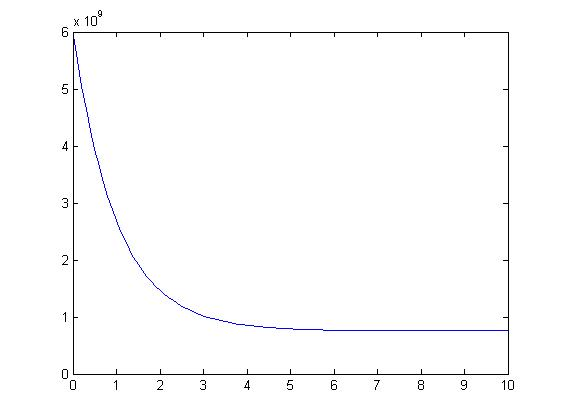
\includegraphics[scale=0.6]{./pic/duiliu.jpg}
%\caption{对流方程的图像,数据取自巨大芽孢杆菌对流方程}\label{pic:duiliu_nnn}
%\end{figure}